\documentclass{article}
\usepackage{graphicx}
\begin{document}
%\title{Reddening Law for Nearby SN Ia}
% \maketitle
\begin{figure}
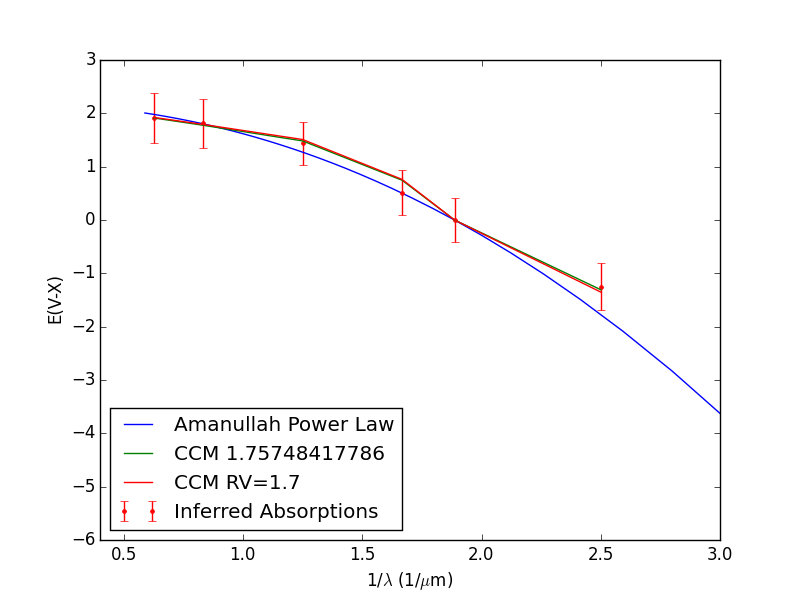
\includegraphics[width=.8\textwidth]{../2014j_redlaw.png}
\caption{SN2014J}
\end{figure}
\begin{figure}
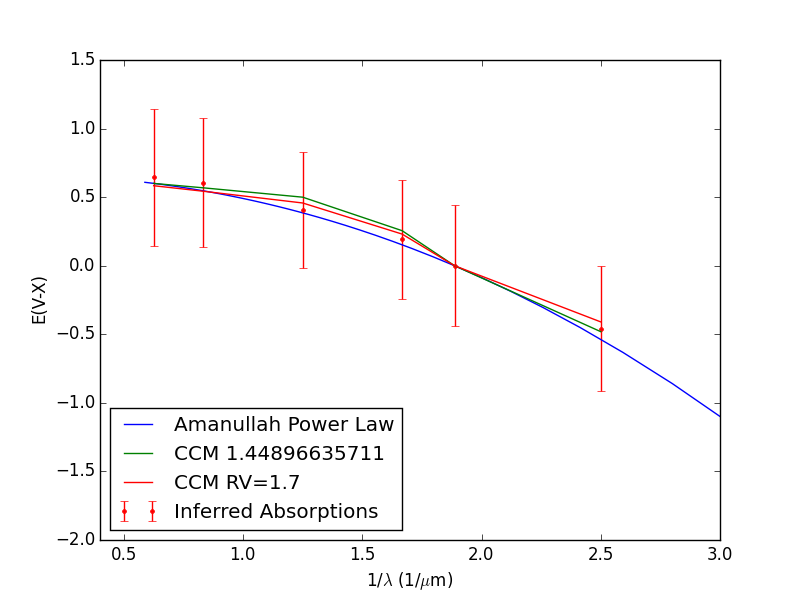
\includegraphics[width=.8\textwidth]{../2007S_redlaw.png}
\caption{SN2007S}
\end{figure}

\begin{figure}
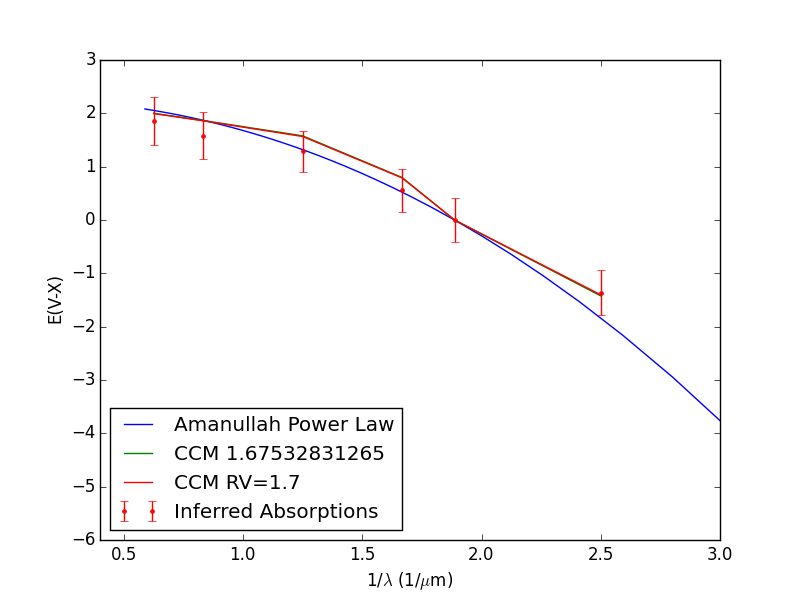
\includegraphics[width=.8\textwidth]{../2006X_redlaw.png}
\caption{SN2006X}
\end{figure}

\begin{figure}
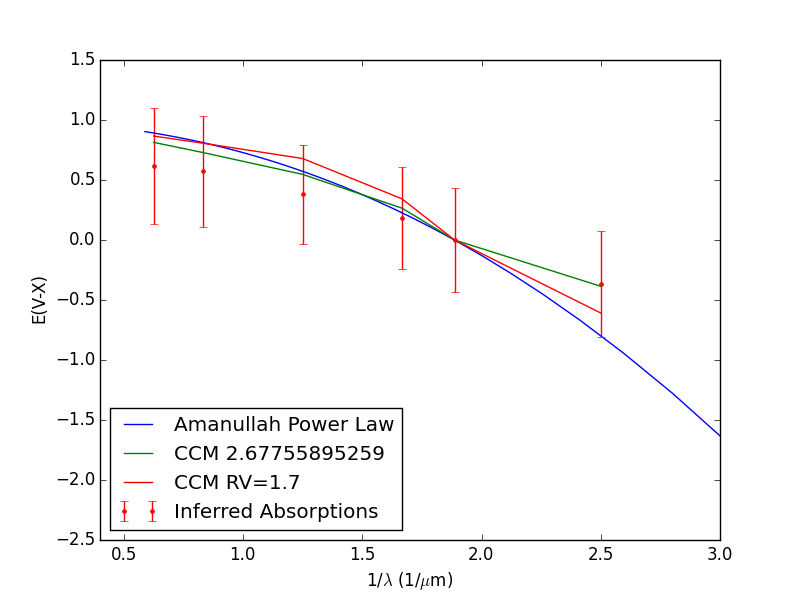
\includegraphics[width=.8\textwidth]{../2007ca_redlaw.png}
\caption{SN2007ca}
\end{figure}

\begin{figure}
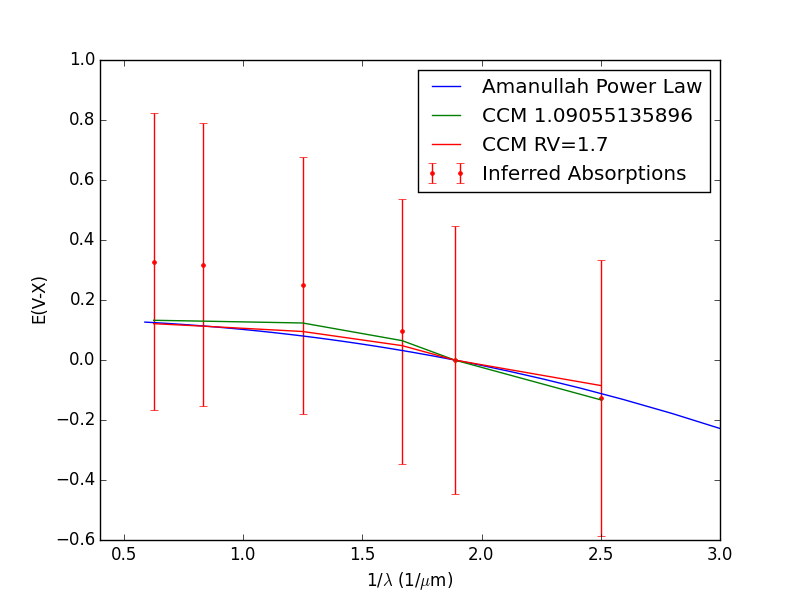
\includegraphics[width=.8\textwidth]{../2004gu_redlaw.png}
\caption{SN2004gu}
\end{figure}
\end{document}

